%!TEX program = xelatex
\documentclass[11pt]{beamer}

\usepackage{amsfonts}
\usepackage{amsmath}
\usepackage{blindtext}
\usepackage{enumitem}
\usepackage{fancyvrb}
\usepackage{tikz}

\usetheme{SaoPaulo}  % can use SaoPaulo as well

\title{MATLAB}
\subtitle{Introduction}
\author{CS101 Lecture \#21}
\date{2016-12-07}

\setcounter{showSlideNumbers}{1}

\newcommand{\correctstar}{{\Large\textcolor{red}{$\star$}}}

\begin{document}
  \setcounter{showProgressBar}{0}
  \setcounter{showSlideNumbers}{0}

%%%%%%%%%%%%%%%%%%%%%%%%%%%%%%%%%%%%%%%%%%%%%%%%%%%%%%%%%%%%%%%%%%%%%%%%%%%%%%%%
\frame{\titlepage}

%%%%%%%%%%%%%%%%%%%%%%%%%%%%%%%%%%%%%%%%%%%%%%%%%%%%%%%%%%%%%%%%%%%%%%%%%%%%%%%%
\setcounter{framenumber}{0}
\setcounter{showProgressBar}{1}
\setcounter{showSlideNumbers}{1}

%%%%%%%%%%%%%%%%%%%%%%%%%%%%%%%%%%%%%%%%%%%%%%%%%%%%%%%%%%%%%%%%%%%%%%%%%%%%%%%%
\section{Administrivia}

%%%%%%%%%%%%%%%%%%%%%%%%%%%%%%%%%%%%%%%%%%%%%%%%%%%%%%%%%%%%%%%%%%%%%%%%%%%%%%%%
\begin{frame}
  \frametitle{Administrivia}
  \Enlarge

   \begin{itemize}
   	\myitem  Homework \#8 is out; 
	\myitem  Due on next Monday, Dec.\ 11th.
   \end{itemize}
\end{frame}

%%%%%%%%%%%%%%%%%%%%%%%%%%%%%%%%%%%%%%%%%%%%%%%%%%%%%%%%%%%%%%%%%%%%%%%%%%%%%%%%
\section{Warmup Quiz}

%%%%%%%%%%%%%%%%%%%%%%%%%%%%%%%%%%%%%%%%%%%%%%%%%%%%%%%%%%%%%%%%%%%%%%%%%%%%%%%%
\begin{frame}[fragile]
  \frametitle{Question \#1}
  \Enlarge

  \begin{Verbatim}
import numpy as np
import math
tmax = 10
dt = 0.01
nt = int( tmax/dt ) + 1
x = np.zeros( (nt,) )
for i in range( 0, tmax, dt ):
    vx = x[ i-1 ] / np.sin( i * math.pi)
    x[ i+1 ] = x[ i ] + vx * dt
  \end{Verbatim}

Which uncaught error will halt this code?

  \begin{enumerate}[label=\Alph*]
    \item  \texttt{ZeroDivisionError}
    \item  \texttt{TypeError}
    \item  \texttt{SyntaxError}
    \item  \texttt{IndexError}
  \end{enumerate}
\end{frame}

%%%%%%%%%%%%%%%%%%%%%%%%%%%%%%%%%%%%%%%%%%%%%%%%%%%%%%%%%%%%%%%%%%%%%%%%%%%%%%%%
\begin{frame}[fragile]
  \frametitle{Question \#1}
  \Enlarge

  \begin{Verbatim}
import numpy as np
import math
tmax = 10
dt = 0.01
nt = int( tmax/dt ) + 1
x = np.zeros( (nt,) )
for i in range( 0, tmax, dt ):
    vx = x[ i-1 ] / np.sin( i * math.py)
    x[ i+1 ] = x[ i ] + vx * dt
  \end{Verbatim}

Which uncaught error will halt this code?

  \begin{enumerate}[label=\Alph*]
    \item  \texttt{ZeroDivisionError}
    \item  \texttt{TypeError}  \correctstar  (\texttt{dt} has to be integer)
    \item  \texttt{SyntaxError}
    \item  \texttt{IndexError}
  \end{enumerate}
\end{frame}

%%%%%%%%%%%%%%%%%%%%%%%%%%%%%%%%%%%%%%%%%%%%%%%%%%%%%%%%%%%%%%%%%%%%%%%%%%%%%%%%
\begin{frame}[fragile]
  \frametitle{Question \#2}
  \Enlarge

  \begin{Verbatim}
x = np.ones( 10 )
for i in range( 10 ):
    try:
        ???
    except Exception:
        print( 'Error on step %d.'%i )
        continue
  \end{Verbatim}

Which of the following candidates for \texttt{???} would \emph{not} produce an error message?

  \begin{enumerate}[label=\Alph*]
    \item  \texttt{x += x[ i+1 ]}
    \item  \texttt{x[ i ] /= 0}
    \item  \texttt{x[ -i-1 ]   = sum( x[ :i ] )}
    \item  \texttt{x[ 10-i ] = sum( x[ :i ] )}
  \end{enumerate}
\end{frame}

%%%%%%%%%%%%%%%%%%%%%%%%%%%%%%%%%%%%%%%%%%%%%%%%%%%%%%%%%%%%%%%%%%%%%%%%%%%%%%%%
\begin{frame}[fragile]
  \frametitle{Question \#2}
  \Enlarge

  \begin{Verbatim}
x = np.ones( 10 )
for i in range( 10 ):
    try:
        ???
    except Exception:
        print( 'Error on step %d.'%i )
        continue
  \end{Verbatim}

Which of the following candidates for \texttt{???} would \emph{not} produce any error message?

  \begin{enumerate}[label=\Alph*]
    \item  \texttt{x += x[ i+1 ]}  \textcolor{red}{index error}
    \item  \texttt{x[ i ] /= 0}  \correctstar (np.dtype('float') handles division by zero without throwing an error)
    \item  \texttt{x[ -i-1 ]   = sum( x[ :i ] )}  \correctstar
    \item  \texttt{x[ 10-i ] = sum( x[ :i ] )}  \textcolor{red}{index error}
  \end{enumerate}
\end{frame}

%%%%%%%%%%%%%%%%%%%%%%%%%%%%%%%%%%%%%%%%%%%%%%%%%%%%%%%%%%%%%%%%%%%%%%%%%%%%%%%%
\section{MATLAB}

%%%%%%%%%%%%%%%%%%%%%%%%%%%%%%%%%%%%%%%%%%%%%%%%%%%%%%%%%%%%%%%%%%%%%%%%%%%%%%%
\begin{frame}[fragile]
  \frametitle{What is MATLAB?}
  \Enlarge

  \begin{enumerate}
  \myitem  Programming language + environment (an IDE).
  \myitem  Proprietary, owned and maintained by MathWorks.
  \myitem  Dates from late 1970s, under active development.
  \myitem  Was an influence on NumPy/matplotlib, so will be familiar.
  \end{enumerate}
\end{frame}


%%%%%%%%%%%%%%%%%%%%%%%%%%%%%%%%%%%%%%%%%%%%%%%%%%%%%%%%%%%%%%%%%%%%%%%%%%%%%%%
\begin{frame}[fragile]
  \frametitle{Why MATLAB?}
  \Enlarge

  \begin{enumerate}
  \myitem  Designed for engineering and scientific computing
  \myitem  Famous for its \emph{matrix-centric} computation
  \myitem  Ideal for:
    \begin{enumerate}
    \mysubitem  Linear algebra
    \mysubitem  Image processing
    \mysubitem  Numerical analysis
    \mysubitem  Simulation, Graphical plot, etc.
    \end{enumerate}
  \myitem  Many toolboxes available.
  \myitem  Excellent documentation:  MATLAB Central.
  \end{enumerate}
\end{frame}

%%%%%%%%%%%%%%%%%%%%%%%%%%%%%%%%%%%%%%%%%%%%%%%%%%%%%%%%%%%%%%%%%%%%%%%%%%%%%%%
\begin{frame}[fragile]
  \frametitle{Basics}
  \Enlarge

  \begin{enumerate}
  \myitem  Literals, variables, operators
  \end{enumerate}
  \begin{Verbatim}
5
  \end{Verbatim}
  \begin{enumerate}
  \myitem  Expressions
  \end{enumerate}
  \begin{Verbatim}
a = 3 * 2
b = 1 + a
  \end{Verbatim}
  \begin{enumerate}
  \myitem  Semicolon suppresses output (mutes):  \texttt{;}
  \end{enumerate}
  \begin{Verbatim}
b = b ^ 2;
  \end{Verbatim}
  \begin{enumerate}
  \myitem  \texttt{ans} is default result.
  \end{enumerate}
  \begin{Verbatim}
a / 4
  \end{Verbatim}
  \begin{enumerate}
  \myitem  \texttt{disp(ans)} displays the value of \texttt{ans}.
  \myitem  \texttt{whos a} shows type, size (as an array), and number of Bytes of  variable \texttt{a} in workspace.
  \end{enumerate}
\end{frame}

%%%%%%%%%%%%%%%%%%%%%%%%%%%%%%%%%%%%%%%%%%%%%%%%%%%%%%%%%%%%%%%%%%%%%%%%%%%%%%%
\begin{frame}[fragile]
  \frametitle{Numeric types}
  \Enlarge

  \begin{enumerate}
  \myitem  MATLAB implements:
    \begin{enumerate}
    \mysubitem  integers
    \mysubitem  floating-point numbers
    \mysubitem  complex numbers
    \mysubitem  logical (boolean, 0/1)
    \end{enumerate}
  \myitem  in 8-, 16-, 32-, and 64-bit versions.
  \end{enumerate}
\end{frame}

%%%%%%%%%%%%%%%%%%%%%%%%%%%%%%%%%%%%%%%%%%%%%%%%%%%%%%%%%%%%%%%%%%%%%%%%%%%%%%%
\begin{frame}[fragile]
  \frametitle{Array types}
  \Enlarge

  \begin{enumerate}
  \myitem  Arrays are the fundamental type in MATLAB:
  \end{enumerate}
  \begin{Verbatim}
a = [ 1 2 3 ];
  \end{Verbatim}
  \begin{enumerate}
  \myitem  Arrays are indexed using parentheses:
  \end{enumerate}
  \begin{Verbatim}
b = a( 1 );
c = a( end );
  \end{Verbatim}
  \begin{enumerate}
  \myitem  \textcolor{red}{MATLAB counts from one, not zero!}
  \end{enumerate}
\end{frame}

%%%%%%%%%%%%%%%%%%%%%%%%%%%%%%%%%%%%%%%%%%%%%%%%%%%%%%%%%%%%%%%%%%%%%%%%%%%%%%%
\begin{frame}[fragile]
  \frametitle{Multidimensional arrays}
  \Enlarge

  \begin{enumerate}
  \myitem  More dimensional arrays use semicolons to separate rows:
  \end{enumerate}
  \begin{Verbatim}
A = [ 1 2 3 ; 4 5 6 ];
  \end{Verbatim}
  \begin{enumerate}
  \myitem  Arrays are indexed using parentheses and commas:
  \end{enumerate}
  \begin{Verbatim}
a = A( 1,2 );
  \end{Verbatim}
  \begin{enumerate}
  \myitem  Helper functions are available:
  \end{enumerate}
  \begin{Verbatim}
B = zeros( 3,3 ) + ones( 3,3 ) + eye( 3,3 ) ;
  \end{Verbatim}
\end{frame}

%%%%%%%%%%%%%%%%%%%%%%%%%%%%%%%%%%%%%%%%%%%%%%%%%%%%%%%%%%%%%%%%%%%%%%%%%%%%%%%%
\begin{frame}[fragile]
  \frametitle{Question}
  \Enlarge
$$
\left(
\begin{array}{ccc}
1 & 1 & 1 \\
2 & 2 & 2
\end{array}
\right)
$$

Which of the following will produce this array?

  \begin{enumerate}[label=\Alph*]
    \item  \texttt{[ 1 1 1 ] ; [ 2 2 2 ]}
    \item  \texttt{[ 1 1 1 ; 2 2 2 ]}
    \item  \texttt{[ 1 2 ] ; [ 1 2 ] ; [ 1 2 ]}
    \item  \texttt{[ 1 2 ; 1 2 ; 1 2 ]}
    \item  \texttt{[ [ 1 1 1 ] , [ 2 2 2 ] ]}
  \end{enumerate}
\end{frame}

%%%%%%%%%%%%%%%%%%%%%%%%%%%%%%%%%%%%%%%%%%%%%%%%%%%%%%%%%%%%%%%%%%%%%%%%%%%%%%%%
\begin{frame}[fragile]
  \frametitle{Question}
  \Enlarge
$$
\left(
\begin{array}{ccc}
1 & 1 & 1 \\
2 & 2 & 2
\end{array}
\right)
$$

Which of the following will produce this array?

  \begin{enumerate}[label=\Alph*]
    \item  \texttt{[ 1 1 1 ] ; [ 2 2 2 ]}
    \item  \texttt{[ 1 1 1 ; 2 2 2 ]} \correctstar
    \item  \texttt{[ 1 2 ] ; [ 1 2 ] ; [ 1 2 ]}
    \item  \texttt{[ 1 2 ; 1 2 ; 1 2 ]}
    \item  \texttt{[ [ 1 1 1 ] , [ 2 2 2 ] ]}
  \end{enumerate}
\end{frame}

%%%%%%%%%%%%%%%%%%%%%%%%%%%%%%%%%%%%%%%%%%%%%%%%%%%%%%%%%%%%%%%%%%%%%%%%%%%%%%%%
\begin{frame}[fragile]
  \frametitle{Question}
  \Enlarge
$$
A =
\left(
\begin{array}{ccc}
1 & 2 & 3 \\
4 & 5 & 6
\end{array}
\right)
$$

Which of the following will access \texttt{4} in this array?

  \begin{enumerate}[label=\Alph*]
    \item  \texttt{A( 1,0 )}
    \item  \texttt{A[ 2,1 ]}
    \item  \texttt{A( 2,1 )}
    \item  \texttt{A( 1 )( 0 )}
  \end{enumerate}
\end{frame}

%%%%%%%%%%%%%%%%%%%%%%%%%%%%%%%%%%%%%%%%%%%%%%%%%%%%%%%%%%%%%%%%%%%%%%%%%%%%%%%%
\begin{frame}[fragile]
  \frametitle{Question}
  \Enlarge
$$
A =
\left(
\begin{array}{ccc}
1 & 2 & 3 \\
4 & 5 & 6
\end{array}
\right)
$$

Which of the following will access \texttt{4} in this array?

  \begin{enumerate}[label=\Alph*]
    \item  \texttt{A( 1,0 )}
    \item  \texttt{A[ 2,1 ]}
    \item  \texttt{A( 2,1 )} \correctstar
    \item  \texttt{A( 1 )( 0 )}
  \end{enumerate}
\end{frame}

%%%%%%%%%%%%%%%%%%%%%%%%%%%%%%%%%%%%%%%%%%%%%%%%%%%%%%%%%%%%%%%%%%%%%%%%%%%%%%%
\begin{frame}[fragile]
  \frametitle{Array operations}
  \Enlarge

  \begin{Verbatim}
% basic mathematics:
A = ( ones( 3,3 ) + 1 ) / 2
B = sin( ones( 3,3 ) * pi )
C = B'  % transpose with '

% matrix multiplication:
D = eye( 3,4 ) * ones( 4,5 )
  \end{Verbatim}
\end{frame}

%%%%%%%%%%%%%%%%%%%%%%%%%%%%%%%%%%%%%%%%%%%%%%%%%%%%%%%%%%%%%%%%%%%%%%%%%%%%%%%%
\begin{frame}[fragile]
  \frametitle{Question}
  \Enlarge
$$
\left(
\begin{array}{cc}
2 & 1 \\
1 & 2
\end{array}
\right)
$$

Which of the following will produce this array?

  \begin{enumerate}[label=\Alph*]
    \item  \texttt{3*ones( 2,2 ) - 2*eye( 2,2 )}
    \item  \texttt{2*ones( 2,2 ) + eye( 2,2 )}
    \item  \texttt{3*ones( 2,2 ) - eye( 2,2 )}
    \item  \texttt{ones( 2,2 ) + eye( 2,2 )}
  \end{enumerate}
\end{frame}

%%%%%%%%%%%%%%%%%%%%%%%%%%%%%%%%%%%%%%%%%%%%%%%%%%%%%%%%%%%%%%%%%%%%%%%%%%%%%%%%
\begin{frame}[fragile]
  \frametitle{Question}
  \Enlarge
$$
\left(
\begin{array}{cc}
2 & 1 \\
1 & 2
\end{array}
\right)
$$

Which of the following will produce this array?

  \begin{enumerate}[label=\Alph*]
    \item  \texttt{3*ones( 2,2 ) - 2*eye( 2,2 )}
    \item  \texttt{2*ones( 2,2 ) + eye( 2,2 )}
    \item  \texttt{3*ones( 2,2 ) - eye( 2,2 )}
    \item  \texttt{ones( 2,2 ) + eye( 2,2 )}  \correctstar
  \end{enumerate}
\end{frame}

%%%%%%%%%%%%%%%%%%%%%%%%%%%%%%%%%%%%%%%%%%%%%%%%%%%%%%%%%%%%%%%%%%%%%%%%%%%%%%%
\begin{frame}[fragile]
  \frametitle{Array operations}
  \Enlarge

  \begin{Verbatim}
% concatenating arrays
A = [  eye( 3,4 ),  eye( 3,5 );
      ones( 2,4 ), ones( 2, 5) ]
  \end{Verbatim}
  \begin{enumerate} \pause
  \myitem horizontal concatenation by ',' or ' '
  \myitem vertical concatenation by  ';'
  \myitem array size must agree!
  \end{enumerate}
\end{frame}

%%%%%%%%%%%%%%%%%%%%%%%%%%%%%%%%%%%%%%%%%%%%%%%%%%%%%%%%%%%%%%%%%%%%%%%%%%%%%%%%
\begin{frame}[fragile]
  \frametitle{Question}
  \Enlarge
$$
\left(
\begin{array}{cc}
1 & 2 \\
3 & 4 \\
5 & 6
\end{array}
\right)
$$

How can we produce this array?

  \begin{enumerate}[label=\Alph*]
    \item  \texttt{[ [ 1 3 5 ] [ 2 4 6 ] ]}
    \item  \texttt{[ [ 1 2 ] [ 3 4 ] [ 5 6 ] ]}
    \item  \texttt{[ [ 1 3 5 ] ; [ 2 4 6 ] ]}
    \item  \texttt{[ [ 1 2 ] ; [ 3 4 ] ; [ 5 6 ] ]}
  \end{enumerate}
\end{frame}

%%%%%%%%%%%%%%%%%%%%%%%%%%%%%%%%%%%%%%%%%%%%%%%%%%%%%%%%%%%%%%%%%%%%%%%%%%%%%%%%
\begin{frame}[fragile]
  \frametitle{Question}
  \Enlarge
$$
\left(
\begin{array}{cc}
1 & 2 \\
3 & 4 \\
5 & 6
\end{array}
\right)
$$

How can we produce this array?

  \begin{enumerate}[label=\Alph*]
    \item  \texttt{[ [ 1 3 5 ] [ 2 4 6 ] ]}
    \item  \texttt{[ [ 1 2 ] [ 3 4 ] [ 5 6 ] ]}
    \item  \texttt{[ [ 1 3 5 ] ; [ 2 4 6 ] ]}
    \item  \texttt{[ [ 1 2 ] ; [ 3 4 ] ; [ 5 6 ] ]} \correctstar
  \end{enumerate}
\end{frame}

%%%%%%%%%%%%%%%%%%%%%%%%%%%%%%%%%%%%%%%%%%%%%%%%%%%%%%%%%%%%%%%%%%%%%%%%%%%%%%%
\begin{frame}[fragile]
  \frametitle{Matrix v. element operations}
  \Enlarge

  %\begin{enumerate}
  %\myitem  ``Matrix dimensions must agree.''
  %\myitem  It is sometimes necessary to distinguish \emph{elementwise} operations and \emph{matrix} operations. %\pause
  %\end{enumerate}
  \begin{Verbatim}
A = 2 * ones( 2,2 )
B = A * eye( 2,2 )  %matrix multiplication  
C = A .* eye( 2,2 ) %elementwise multiply
  \end{Verbatim}
  \begin{enumerate}
  \myitem  Denoted by the dot \texttt{.} in front of the operator.
  \myitem  Matrix dimensions must agree. %We won't emphasize this but frequently you must distinguish.
  \end{enumerate}
\end{frame}


%%%%%%%%%%%%%%%%%%%%%%%%%%%%%%%%%%%%%%%%%%%%%%%%%%%%%%%%%%%%%%%%%%%%%%%%%%%%%%%%
\section{Scripts and Function}


%%%%%%%%%%%%%%%%%%%%%%%%%%%%%%%%%%%%%%%%%%%%%%%%%%%%%%%%%%%%%%%%%%%%%%%%%%%%%%%
\begin{frame}[fragile]
  \frametitle{Scripting}
  \Enlarge

  \begin{enumerate}
  \myitem  MATLAB uses \texttt{.m} files for two purposes:  scripts and functions.
  \myitem  Use the built-in editor to create these.
  \myitem Use `\texttt{edit}' command to open or edit a (\texttt{.m}) file from cmd window
  \end{enumerate}
\end{frame}

%%%%%%%%%%%%%%%%%%%%%%%%%%%%%%%%%%%%%%%%%%%%%%%%%%%%%%%%%%%%%%%%%%%%%%%%%%%%%%%
\begin{frame}[fragile]
  \frametitle{Run a script}
  \Enlarge

  \begin{enumerate}
  \myitem  Scripts contain a sequence of commands to run %, like \texttt{.py} scripts.
  \myitem  From command window: \texttt{filename} (no '\texttt{.m}')
  %\myitem  start matlab in your terminal: \texttt{matlab -nodesktop} 
  	%\begin{enumerate}
  %\myitem Open matlab in terminal without the graphical interface: \texttt{matlab -nodesktop}
	%\end{enumerate}
  %\begin{enumerate}
  %\mysubitem  {\small Make sure matlab can be located from your system PATH}
  \myitem  { Be aware of your Present Working Directory (\texttt{pwd}).}
  %\end{enumerate}
  \myitem Use \texttt{addpath} and \texttt{genpath} to add folder/sub-folders to your search paths.
  \end{enumerate}
\end{frame}

%%%%%%%%%%%%%%%%%%%%%%%%%%%%%%%%%%%%%%%%%%%%%%%%%%%%%%%%%%%%%%%%%%%%%%%%%%%%%%%
\begin{frame}[fragile]
  \frametitle{Functions}
  \Enlarge

  \begin{enumerate}
  \myitem  A function must be defined in a file of the same name.
  \end{enumerate}
  \begin{Verbatim}
function [outputs] = function_name(inputs)
    % ...
    % ...
end
  \end{Verbatim}
  \begin{enumerate}
  \myitem Multiple input/output variables separated by \texttt{','} 
  \myitem No explicit \texttt{return} statements
  \myitem  Takes the value of output variable(s) that is produced in the function
  \end{enumerate}
\end{frame}



%%%%%%%%%%%%%%%%%%%%%%%%%%%%%%%%%%%%%%%%%%%%%%%%%%%%%%%%%%%%%%%%%%%%%%%%%%%%%%%
\begin{frame}[fragile]
  \frametitle{Functions}
  \Enlarge

$$
T_{\text{C}} = \frac{100}{180} (T_{\text{F}} - 32) 
$$

File \texttt{CelsiusFromFahrenheit.m}:
  \begin{Verbatim}
function Tc = CelsiusFromFahrenheit(Tf)
    Tc = (Tf - 32) * ( 100/180 );
end
  \end{Verbatim}
\end{frame}

%%%%%%%%%%%%%%%%%%%%%%%%%%%%%%%%%%%%%%%%%%%%%%%%%%%%%%%%%%%%%%%%%%%%%%%%%%%%%%%
\begin{frame}[fragile]
  \frametitle{Commenting in scripts}
  \Enlarge

  \begin{enumerate}
  \myitem  Comments are indicated as follows:
  \end{enumerate}
  \begin{Verbatim}
% this is a comment
%{
  this 
  is 
  a 
  block comment
%}
  \end{Verbatim}
\end{frame}

\iffalse
%%%%%%%%%%%%%%%%%%%%%%%%%%%%%%%%%%%%%%%%%%%%%%%%%%%%%%%%%%%%%%%%%%%%%%%%%%%%%%%
\begin{frame}[fragile]
  \frametitle{Matrix multiplication}
  \Enlarge
  \begin{tikzpicture}[remember picture]
  \node[at=(current page.center)] {
                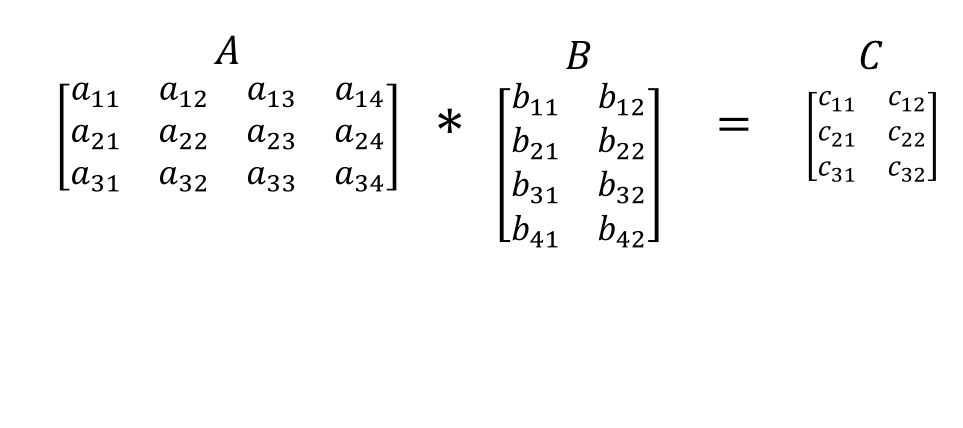
\includegraphics[height=0.4\paperheight]{./img/mult1.png}
            };
  \end{tikzpicture}
\end{frame}

%%%%%%%%%%%%%%%%%%%%%%%%%%%%%%%%%%%%%%%%%%%%%%%%%%%%%%%%%%%%%%%%%%%%%%%%%%%%%%%
\begin{frame}[fragile]
  \frametitle{Matrix multiplication}
  \Enlarge
  \begin{tikzpicture}[remember picture]
  \node[at=(current page.center)] {
                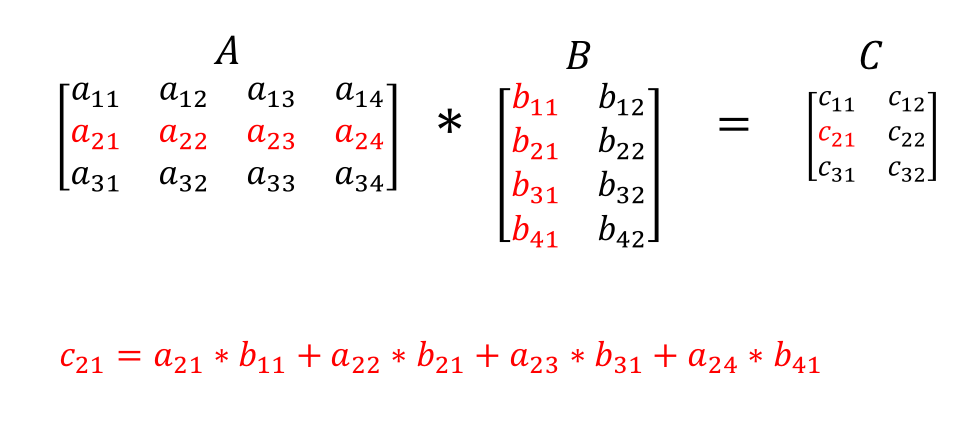
\includegraphics[height=0.4\paperheight]{./img/mult2.png}
            };
  \end{tikzpicture}
\end{frame}

\fi

%%%%%%%%%%%%%%%%%%%%%%%%%%%%%%%%%%%%%%%%%%%%%%%%%%%%%%%%%%%%%%%%%%%%%%%%%%%%%%%
\begin{frame}[fragile]
  \frametitle{Strings}
  \Enlarge

  \begin{enumerate}
  \myitem  Also supports strings, not as convenient as numbers (python is a better choice for handling strings) \pause
  \myitem Manages string as an array of the '\texttt{char}' type \pause
  \myitem  Enclosed with single quotes (only!).
  \end{enumerate}
  
  \begin{Verbatim}
   s = 'a brown fox';
   class(s)
   size(s)
  \end{Verbatim}
\end{frame}

%%%%%%%%%%%%%%%%%%%%%%%%%%%%%%%%%%%%%%%%%%%%%%%%%%%%%%%%%%%%%%%%%%%%%%%%%%%%%%%
\begin{frame}[fragile]
  \frametitle{String formating and print}
  \Enlarge

  \begin{enumerate}
  \myitem  Print formatted strings with \texttt{sprintf}, \texttt{fprintf}
  \end{enumerate}
  \begin{Verbatim}
s = sprintf( '%d %f\n', 5, sin(pi/4) ); 

%output to screen
fprintf('%d %f\n', 5, sin(pi/4)); 

%output to file
fp = fopen('newfile.txt', 'w')
fprintf(fp, '%d %f\n', 5, sin(pi/3));
fclose(fp)
\end{Verbatim}
\end{frame}


\begin{frame}[fragile]
  \frametitle{Look for more information}
  \Enlarge

  \begin{enumerate}
    \myitem  help \texttt{fprintf}   
    	\begin{enumerate}
	\mysubitem displays help information to the screen
	\end{enumerate}
    \myitem  doc \texttt{fprintf}   
    	\begin{enumerate}
	\mysubitem opens matlab's documentation book
	\end{enumerate}\pause
  \end{enumerate}
  

  \vspace{5mm}
  Tutorial: {\small \url{http://zichengl.net/cmpt469/matlabtutorial.m}}
  
\end{frame} 
\end{document}
